\documentclass{beamer}

\usetheme{CambridgeUS}

\usepackage[utf8]{inputenc}
\usepackage[T1]{fontenc}

\usepackage{CJKutf8}
\usepackage{datetime}
\usepackage{amsmath}
\usepackage{amssymb}
\usepackage{mathtools}
\usepackage{subcaption}
\usepackage{xcolor}
\usepackage{tikz}

\usetikzlibrary{positioning, quotes}

\newdate{date}{21}{04}{2023}
\date{\displaydate{date}}
\title[SAT]{The Why, How, and What of SAT}
\author[Rex]{\begin{CJK}{UTF8}{bsmi}袁至誠\end{CJK}\\Chih-cheng Rex Yuan}
\institute[at SZU]{Shenzhen University}

\usetikzlibrary{arrows,shapes,fit}
\pgfdeclarelayer{background}
\pgfsetlayers{background,main}

\DeclarePairedDelimiter{\set}{\{}{\}}
\DeclarePairedDelimiter{\tuple}{(}{)}
\DeclarePairedDelimiter{\abs}{\lvert}{\rvert}

\let\oldleq\leq
\renewcommand{\leq}[1][]{\oldleq_{#1}}
\renewcommand{\implies}{\rightarrow}

\newcommand{\bye}[1]{}
\newcommand{\bicond}{\leftrightarrow}
\newcommand{\poset}[1]{\mathcal{#1}}
\newcommand{\uni}[1][]{\Omega_{#1}}
\newcommand{\lang}[1]{L(#1)}
\newcommand{\lin}[1]{\texttt{#1}}
\newcommand{\swap}[1][]{\leftrightarrow_{#1}}
\newcommand{\sgraph}[1]{G(#1)}
\newcommand{\lext}{\sqsubseteq}
\newcommand{\incomp}[1][]{\parallel_{#1}}
\newcommand{\covered}[1][]{\prec_{#1}}
\newcommand{\complmt}[1]{\overline{#1}}
\newcommand{\satvar}[2]{\mathtt{X}_{#1}^{#2}}
\newcommand{\bigo}[1]{\mathcal{O}(#1)}
\newcommand{\code}[1]{\texttt{#1}}
\newcommand{\swapfn}[2]{#1[#2]}
\newcommand{\inv}[2]{inv(#1,#2)}

\begin{document}

\begin{frame}
\titlepage
\end{frame}

\begin{frame}
    \frametitle{P and NP}
    \alert{P} The class of problems that are ``easy'':
    \begin{itemize}
        \item $\bigo{1}$
        \item $\bigo{n}$
        \item $\bigo{n^3 + k}$
    \end{itemize}

    \alert{NP} The class of problems that are ``hard'':
    \begin{itemize}
        \item $\bigo{n!}$
        \item $\bigo{2^n}$
        \item $\bigo{2^{n^3+k}}$
    \end{itemize}

    For all intents and purposes, P $\neq$ NP.
\end{frame}

\begin{frame}
    \frametitle{Hamiltonian path}
    A Hamiltonian path of a graph is a path which visits every
    node of the graph exactly once.

    A Hamiltonian path of $G$ is $\tuple{a,b,d,c}$.
    \begin{figure}[H]
        \centering
        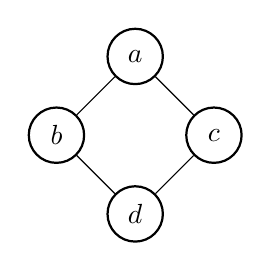
\begin{tikzpicture}
            [
            vertex/.style={circle,thick,draw,minimum size=2em},
            edge/.style={}
            ]
        \node[vertex] (1) at (1,2) {$a$};
        \node[vertex] (2) at (0,1) {$b$};
        \node[vertex] (3) at (2,1) {$c$};
        \node[vertex] (4) at (1,0) {$d$};
        \draw[edge] (1) -- (2);
        \draw[edge] (1) -- (3);
        \draw[edge] (2) -- (4);
        \draw[edge] (3) -- (4);
        \end{tikzpicture}
        \caption{Undirected $\sgraph{\set{a,b,c,d}, E}$}
        \label{figure:posetp}
    \end{figure}

    A Hamiltonian path can be found in $\bigo{n \times n!}$ by enumerating
    over all possible sequence and checking each of them if it is a path.
\end{frame}

\begin{frame}
    \frametitle{Hardness, Completeness, and Reduction}
    \alert{Reduction} A reduction is a problem ``wrapper''.
    We say $A$ reduces to $B$ if there's an ``easy enough''
    reduction $R$ such that we can solve $A$ by passing
    the input through $R$ to $B$.

    \begin{figure}[H]
        \centering
        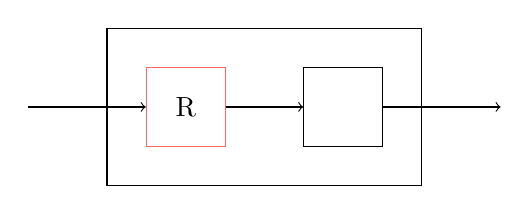
\begin{tikzpicture}
        \draw[draw=black] (0,0) rectangle (4,2);
        \node[draw=red!60,rectangle,minimum size=10mm] (R) at (1,1) {R};
        \node[draw,rectangle,minimum size=10mm] (B) at (3,1) {};
        \draw[->] (R) -- (B);
        \draw[->] (-1,1) -- (R);
        \draw[->] (B) -- (5,1);
        \end{tikzpicture}
    \end{figure}

    \alert{Hardness} If every problem of a class $C$ reduces to a
    problem $A$, we say that $A$ is $C$-hard.

    \alert{Completeness} If $A$ is $C$-hard and $A$ is also in the class $C$,
    we say that $A$ is $C$-complete.
    \\~\\
    A $C$-complete problem can be treated as the ``hardest'' problem in that class.
\end{frame}

\begin{frame}
    \frametitle{Why SAT?}
    \begin{block}{Fact}
        Hamiltonian path is NP-complete.
    \end{block}
    Solving Hamiltonian path is tough.
    \begin{block}{Fact}
        SAT is NP-complete.
    \end{block}
    Solving SAT is also tough, but since it's NP-complete,
    if we can solve it fairly fast, we can solve any NP problem
    fairly fast.
    \\~\\
    However, decades of research in SAT-solving has yielded heuristics
    and implementations that are ``unreasonably effective'' against
    large problems (millions of clauses and variables).
\end{frame}

\begin{frame}
    \frametitle{Reduction of Hamiltonian path to SAT}
    $G=\tuple{S,E}$. Set $\satvar{i,j}{}$ to mean
    the $i$th position in the Hamiltonian path is
    occupied by node $j$.
    \begin{itemize}
        \item Each node $j$ must appear in the path:
        $\bigwedge_{j \in S} \bigvee_{i \in S} \satvar{i,j}{}$
        \item No node $j$ appears twice in the path:
        $\bigwedge_{i,j,k \in S, i \neq k} \neg (\satvar{i,j}{} \wedge \satvar{k,j}{})$
        \item Every position $i$ on the path must be occupied:
        $\bigwedge_{i \in S} \bigvee_{j \in S} \satvar{i,j}{}$
        \item No two nodes $j$ and $k$ occupy the same position in the path:
        $\bigwedge_{i,j,k \in S, j \neq k} \neg (\satvar{i,j}{} \wedge \satvar{i,k}{})$
        \item Nonadjacent nodes i and j cannot be adjacent in the path:
        $\bigwedge_{k \in \set{1,...,n-1}, (i,j) \notin E} \neg (\satvar{k,i}{} \wedge \satvar{k+1,j}{})$
    \end{itemize}
\end{frame}

\begin{frame}
    \frametitle{How SAT?}
    The backbone of modern SAT-solving is the idea of unit propagration and
    Conflict-Driven Clause-Learning (CDCL). Consider this example
    from Carsten Sinz and Tomáš Balyo of Karlsruhe Institute of Technology.

    \begin{columns}
    \column{0.6\textwidth}
    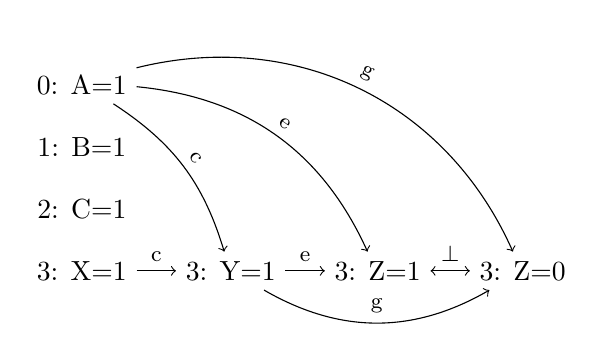
\begin{tikzpicture}
        [
        every edge quotes/.style = {auto, font=\footnotesize, sloped}
        ]
    \node[] (a) {0: A=1};
    \node[below=0.3cm of a] (b) {1: B=1};
    \node[below=0.3cm of b] (c) {2: C=1};
    \node[below=0.3cm of c] (x) {3: X=1};
    \node[right=0.5cm of x] (y) {3: Y=1};
    \node[right=0.5cm of y] (z) {3: Z=1};
    \node[right=0.5 of z] (nz) {3: Z=0};

    \draw[->] (a) edge["c", bend left=20] (y);
    \draw[->] (x) edge["c"] (y);
    \draw[->] (a) edge["e", bend left=30] (z);
    \draw[->] (y) edge["e"] (z);
    \draw[->] (a) edge["g", bend left=40] (nz);
    \draw[->] (y) edge["g", bend right=30] (nz);
    \draw[<->] (z) edge["$\bot$"] (nz);
    \end{tikzpicture}

    \column{0.4\textwidth}
    \begin{align*}
     \{ & \set{A,B},                      && a \\
        & \set{B,C},                      && b \\
        & \set{\neg A, \neg X, Y},        && c \\
        & \set{\neg A, X, Z},             && d \\
        & \set{\neg A, \neg Y, Z},        && e \\
        & \set{\neg A, X, \neg Z},        && f \\
        & \set{\neg A, \neg Y, \neg Z} \} && g \\
    \end{align*}
    \end{columns}
\end{frame}

\begin{frame}
    \frametitle{CDCL}
    \begin{columns}
    \column{0.6\textwidth}
    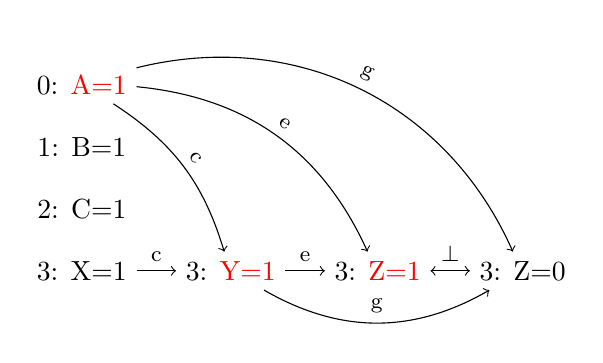
\begin{tikzpicture}
        [
        every edge quotes/.style = {auto, font=\footnotesize, sloped}
        ]
    \node[] (a) {0: {\color{red} A=1}};
    \node[below=0.3cm of a] (b) {1: B=1};
    \node[below=0.3cm of b] (c) {2: C=1};
    \node[below=0.3cm of c] (x) {3: X=1};
    \node[right=0.5cm of x] (y) {3: {\color{red} Y=1}};
    \node[right=0.5cm of y] (z) {3: {\color{red} Z=1}};
    \node[right=0.5 of z] (nz) {3: Z=0};

    \draw[->] (a) edge["c", bend left=20] (y);
    \draw[->] (x) edge["c"] (y);
    \draw[->] (a) edge["e", bend left=30] (z);
    \draw[->] (y) edge["e"] (z);
    \draw[->] (a) edge["g", bend left=40] (nz);
    \draw[->] (y) edge["g", bend right=30] (nz);
    \draw[<->] (z) edge["$\bot$"] (nz);
    \end{tikzpicture}

    \column{0.4\textwidth}
    \begin{align*}
     \{ & \set{A,B},                      && a \\
        & \set{B,C},                      && b \\
        & \set{\neg A, \neg X, Y},        && c \\
        & \set{\neg A, X, Z},             && d \\
        & \set{\neg A, \neg Y, Z},        && e \\
        & \set{\neg A, X, \neg Z},        && f \\
        & \set{\neg A, \neg Y, \neg Z} \} && g \\
    \end{align*}
    \end{columns}
    Conflicting clause: $\neg (A \wedge Y \wedge Z) =
    {\color{red} \set{\neg A, \neg Y, \neg Z}}$
    \\~\\
    By adding this ``learned'' clause to our database,
    we prevent all future cases where this conflict
    may arise again.
\end{frame}

\begin{frame}
    \frametitle{Much, much more optimization}
    All aspects of SAT algorithms have been studied and analyzed
    extensively.
    Choice heuristics and efficient data structure
    have been developed for decision variable
    branching,
    learned clause cut selection, clause management
    , clause watching, clause reduction, assignment trail recording,
    random restarting, preprocessing, etc.
\end{frame}

\begin{frame}
\frametitle{What SAT}
Here I will present a practical application of SAT solving an NP complete problem.
\begin{figure}[H]
    % figure:cover example c
    \begin{subfigure}[b]{0.5\textwidth}
        \centering
        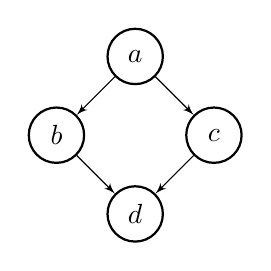
\begin{tikzpicture}
            [
            vertex/.style={circle,thick,draw,minimum size=2em},
            edge/.style={->,> = latex'}
            ]
        \node[vertex] (1) at (1,2) {$a$};
        \node[vertex] (2) at (0,1) {$b$};
        \node[vertex] (3) at (2,1) {$c$};
        \node[vertex] (4) at (1,0) {$d$};
        \draw[edge] (1) -- (2);
        \draw[edge] (1) -- (3);
        \draw[edge] (2) -- (4);
        \draw[edge] (3) -- (4);
        \end{tikzpicture}
    \end{subfigure}%
    % figure:cover example c'
    \begin{subfigure}[b]{0.5\textwidth}
        \centering
        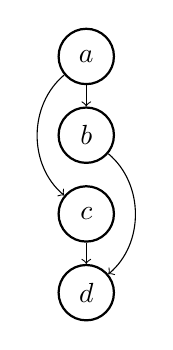
\begin{tikzpicture}
            [
            vertex/.style={circle,thick,draw,minimum size=2em},
            edge/.style={->}
            ]
        \node[vertex] (1) at (0,3) {$a$};
        \node[vertex] (2) at (0,2) {$b$};
        \node[vertex] (3) at (0,1) {$c$};
        \node[vertex] (4) at (0,0) {$d$};
        \draw[edge] (1) -- (2);
        \draw[->] (1) edge[bend right=50] (3);
        \draw[edge] (3) -- (4);
        \draw[->] (2) edge[bend left=50] (4);
        \end{tikzpicture}
    \end{subfigure}
    \label{figure:cover example}
\end{figure}
For a DAG, a topological sort is an ordering of its vertices
such that if $u$ is before $v$, then there cannot be an edge from
$v$ back to $u$.

An example of a topological sort of the DAG on the left
is $\lin{abcd}$, which is depicted on the right.
\end{frame}

\begin{frame}
\frametitle{Poset cover problem}
The inverse problem of topological sorting is called
the \textbf{poset cover problem}, where a set of linear ordering is given,
and the goal is to find a minimal set of DAGs that can
topological sort out to them.
Given the set of linear ordering
$\set{\lin{abdce},\lin{badce},\lin{abcde},\lin{abdec}}$
, two minimal poset covers of two DAGs are shown below:
\begin{figure}[H]
    % figure:cover example c
    \begin{subfigure}[b]{0.5\textwidth}
        \centering
        \begin{subfigure}[b]{0.3\textwidth}
            \centering
            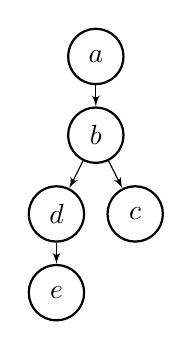
\begin{tikzpicture}
                [
                vertex/.style={circle,thick,draw,minimum size=2em},
                edge/.style={->,> = latex'}
                ]
            \node[vertex] (1) at (1,4) {$a$};
            \node[vertex] (2) at (1,3) {$b$};
            \node[vertex] (3) at (0.5,2) {$d$};
            \node[vertex] (4) at (0.5,1) {$e$};
            \node[vertex] (5) at (1.5,2) {$c$};
            \draw[edge] (1) -- (2);
            \draw[edge] (2) -- (3);
            \draw[edge] (3) -- (4);
            \draw[edge] (2) -- (5);
            \end{tikzpicture}
        \end{subfigure}%
        \begin{subfigure}[b]{0.3\textwidth}
            \centering
            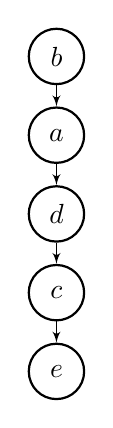
\begin{tikzpicture}
                [
                vertex/.style={circle,thick,draw,minimum size=2em},
                edge/.style={->,> = latex'}
                ]
            \node[vertex] (6) at (4,4) {$b$};
            \node[vertex] (7) at (4,3) {$a$};
            \node[vertex] (8) at (4,2) {$d$};
            \node[vertex] (9) at (4,1) {$c$};
            \node[vertex] (10) at (4,0) {$e$};
            \draw[edge] (6) -- (7);
            \draw[edge] (7) -- (8);
            \draw[edge] (8) -- (9);
            \draw[edge] (9) -- (10);
            \end{tikzpicture}
        \end{subfigure}
    \end{subfigure}%
    % figure:cover example c'
    \begin{subfigure}[b]{0.5\textwidth}
        \centering
        \begin{subfigure}[b]{0.3\textwidth}
            \centering
            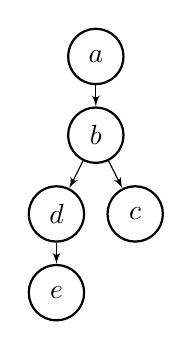
\begin{tikzpicture}
                [
                vertex/.style={circle,thick,draw,minimum size=2em},
                edge/.style={->,> = latex'}
                ]
            \node[vertex] (1) at (1,4) {$a$};
            \node[vertex] (2) at (1,3) {$b$};
            \node[vertex] (3) at (0.5,2) {$d$};
            \node[vertex] (4) at (0.5,1) {$e$};
            \node[vertex] (5) at (1.5,2) {$c$};
            \draw[edge] (1) -- (2);
            \draw[edge] (2) -- (3);
            \draw[edge] (3) -- (4);
            \draw[edge] (2) -- (5);
            \end{tikzpicture}
        \end{subfigure}%
        \begin{subfigure}[b]{0.3\textwidth}
            \centering
            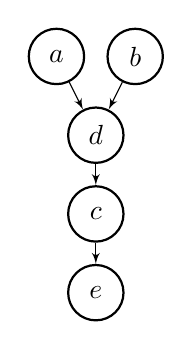
\begin{tikzpicture}
                [
                vertex/.style={circle,thick,draw,minimum size=2em},
                edge/.style={->,> = latex'}
                ]
            \node[vertex] (6) at (3.5,4) {$a$};
            \node[vertex] (7) at (4.5,4) {$b$};
            \node[vertex] (8) at (4,3) {$d$};
            \node[vertex] (9) at (4,2) {$c$};
            \node[vertex] (10) at (4,1) {$e$};
            \draw[edge] (6) -- (8);
            \draw[edge] (7) -- (8);
            \draw[edge] (8) -- (9);
            \draw[edge] (9) -- (10);
            \end{tikzpicture}
        \end{subfigure}
    \end{subfigure}
\end{figure}
\end{frame}

\begin{frame}
    \frametitle{Reduction of poset cover problem to SAT}
    For a DAG $\poset{P}$ and $x \!\neq\! y \!\in\! \uni$,
    we encode with the propositional variable
    $\satvar{x,y}{\poset{P}}$ the case that
    there is a path from
    $x$ to $y$. We
    must first set some constraints based on the axioms
    of the DAG properties.
    \begin{itemize}
        \item Two distinct nodes can't have paths both ways:
        $
        \bigwedge_{x \neq y \in \uni} \neg (\satvar{x,y}{\poset{P}} \wedge \satvar{y,x}{\poset{P}})
        $
        \item If $x$ leads to $y$ and $y$ leads to $z$
        then it must be that $x$ leads to $z$:
        $
        \bigwedge_{x \neq y \neq z \in \uni}
        \satvar{x,y}{\poset{P}} \wedge \satvar{y,z}{\poset{P}} \implies \satvar{x,z}{\poset{P}}
        $
        \item Moreover, for a linear DAG, we have
        on top of that:
        $
        \bigwedge_{x \neq y \in \uni} \satvar{x,y}{\poset{P}} \vee \satvar{y,x}{\poset{P}}
        $
    \end{itemize}
    If a DAG $\poset{P}$ have a topological sort $\poset{L}$,
    we denote that $\poset{P} \lext \poset{L}$, and this property
    is encoded by the constraints:
    \[
    \poset{P} \lext \poset{L} \coloneqq
    \bigwedge_{x \neq y \in \uni} \satvar{x,y}{\poset{P}}
    \implies \satvar{x,y}{\poset{L}}
    \]
\end{frame}

\begin{frame}
    \frametitle{Reduction of poset cover problem to SAT}
    \begin{block}{Poset cover problem}
        Given a set of linear DAGs $\Upsilon$,
        find a set of DAGs $C$, called a cover,
        such that $\abs{C}$ is minimal and the union
        of the topological sorts of DAGs in $C$ is equal
        to $\Upsilon$; that is,
        $\Upsilon = \bigcup_{\poset{P} \in C} \lang{\poset{P}}$
        , where $L$ denotes the set of topological sorts of a DAG.
    \end{block}
    We can reduce the poset cover problem to SAT and set $\abs{C}$
    incrementally from 1 to find the minimal cover, but for the equality
    $\Upsilon = \bigcup_{\poset{P} \in C} \lang{\poset{P}}$ to hold,
    we must have by definition that
    $\Upsilon \subseteq \bigcup_{\poset{P} \in C} \lang{\poset{P}}$
    and
    $\Upsilon \supseteq \bigcup_{\poset{P} \in C} \lang{\poset{P}}$.
\end{frame}

\begin{frame}
    \frametitle{Reduction of poset cover problem to SAT}
    A naive reduction is to encode
    \[
    \Upsilon \subseteq \bigcup_{\poset{P} \in C} \lang{\poset{P}}
    \]
    as
    \[
    \bigwedge_{\poset{L} \in \Upsilon} \bigvee_{\poset{P} \in C} \poset{P} \lext \poset{L}
    \]
    and
    \[
    \Upsilon \supseteq \bigcup_{\poset{P} \in C} \lang{\poset{P}}
    \]
    as
    \[
    \bigwedge_{\poset{L} \in \complmt{\Upsilon}} \bigwedge_{\poset{P} \in C} \poset{P} \not\lext \poset{L}
    \]
    But this latter case causes exponential blowup
    because $\abs{\complmt{\Upsilon}} \in \bigo{n!}$.
\end{frame}

\begin{frame}
    \frametitle{Reduction of poset cover problem to SAT}
    A better encoding is needed. It also necesarrily exists
    because poset cover problem was proved to be NP-complete.
    \begin{block}{Definition}
    The \emph{adjacent transposition}, or \emph{swap},
    relation $\swap$ describes the case of ``off by one swap''
    between linear DAGs with shared universe: for linear DAGs
    $\poset{L}_1,\poset{L}_2$, we denote this relation by
    $\poset{L}_1 \swap \poset{L}_2$
    \end{block}
    An example of this is $\lin{abcd} \swap \lin{acbd}$.
\end{frame}

\begin{frame}
    \frametitle{Reduction of poset cover problem to SAT}
    \begin{block}{Definition}
    For a set of linear DAGs $\Upsilon$,
    the \emph{swap graph} $\sgraph{\Upsilon}$ of it is
    the undirected graph $\tuple{V,E} = \tuple{\Upsilon,\swap}$.
    \end{block}
    The swap graph of the previous example $\lin{abcd} \swap \lin{acbd}$ is:
    \begin{figure}[H]
        \centering
        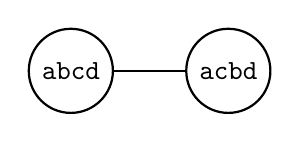
\begin{tikzpicture}
            [
            vertex/.style={circle,thick,draw,minimum size=2em},
            edge/.style={thick}
            ]
        \node[vertex] (1) at (0,0) {\lin{abcd}};
        \node[vertex] (2) at (2,0) {\lin{acbd}};
        \draw[edge] (1) -- (2);
        \end{tikzpicture}
        \label{figure:graphlp}
    \end{figure}
    \begin{block}{Observation}
    A swap graph built from the topological sorts
    of a DAG is connected.
    \end{block}
    We will exploit this observation for our better reduction.
\end{frame}

\begin{frame}
    \frametitle{Reduction of poset cover problem to SAT}
    We ``insulate'' each closed connected component
    $\upsilon \subseteq \sgraph{\Upsilon}$ with a
    ``moat'' set. We denote by $moat(\Upsilon)$ the union of
    the moat sets.

    \begin{figure}[H]
        %\centering
        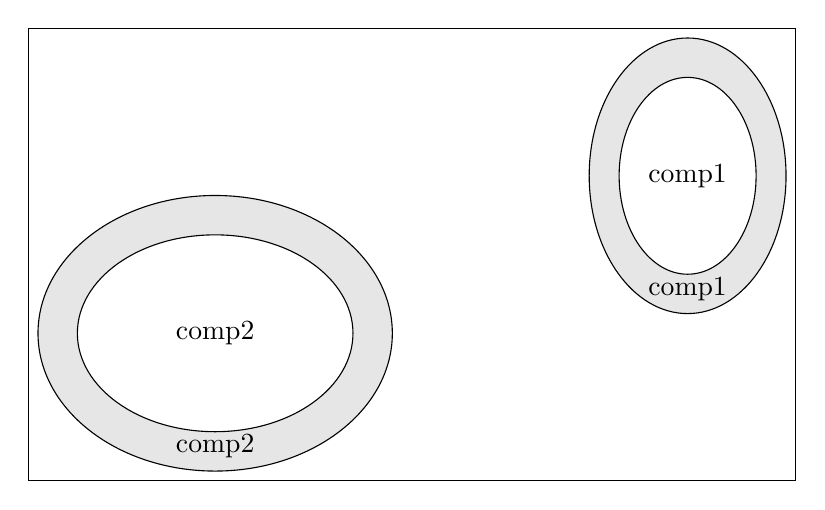
\begin{tikzpicture}
            \node[draw,ellipse,minimum height=2.5cm,minimum width=1.5cm,fill=white] (comp1) at (8,4) {comp1};

            \node[draw,ellipse,minimum height=2.5cm,minimum width=3.5cm,fill=white] (comp2) at (2,2) {comp2};

            \begin{pgfonlayer}{background}
                \node[draw,ellipse,minimum height=3.5cm,minimum width=2.5cm,fill=gray,fill opacity=0.2,text opacity=1] (comp1moat) at (8,4) {};
                \node[above=0.5mm] at (comp1moat.south) {comp1};

                \node[draw,ellipse,minimum height=3.5cm,minimum width=4.5cm,fill=gray,fill opacity=0.2,text opacity=1] (comp2moat) at (2,2) {};
                \node[above=0.5mm] at (comp2moat.south) {comp2};
            \end{pgfonlayer}

            \node[draw,fit=(comp1moat)(comp2moat)] (x) {};
        \end{tikzpicture}
    \end{figure}
\end{frame}

\begin{frame}
    \frametitle{Reduction of poset cover problem to SAT}
    With this information, an alternative way to encode
    $\Upsilon \supseteq \bigcup_{\poset{P} \in C}
    \lang{\poset{P}}$ is:
    \[
    \bigwedge_{\poset{L} \in moat(\Upsilon)}
    \bigwedge_{\poset{P} \in C} \poset{P} \not\lext \poset{L}
    \]
    And we have found our reduction.
\end{frame}

\begin{frame}
    \frametitle{The end}
    The source code of this slides is available at:
    \url{https://github.com/RexYuan/Henwick/blob/master/slides/2023_4_21.tex}
    \\~\\
    Questions?
\end{frame}

\end{document}
